\section{Qualitative Analysis}
\label{sec:discussion}

\begin{figure*}[ht]
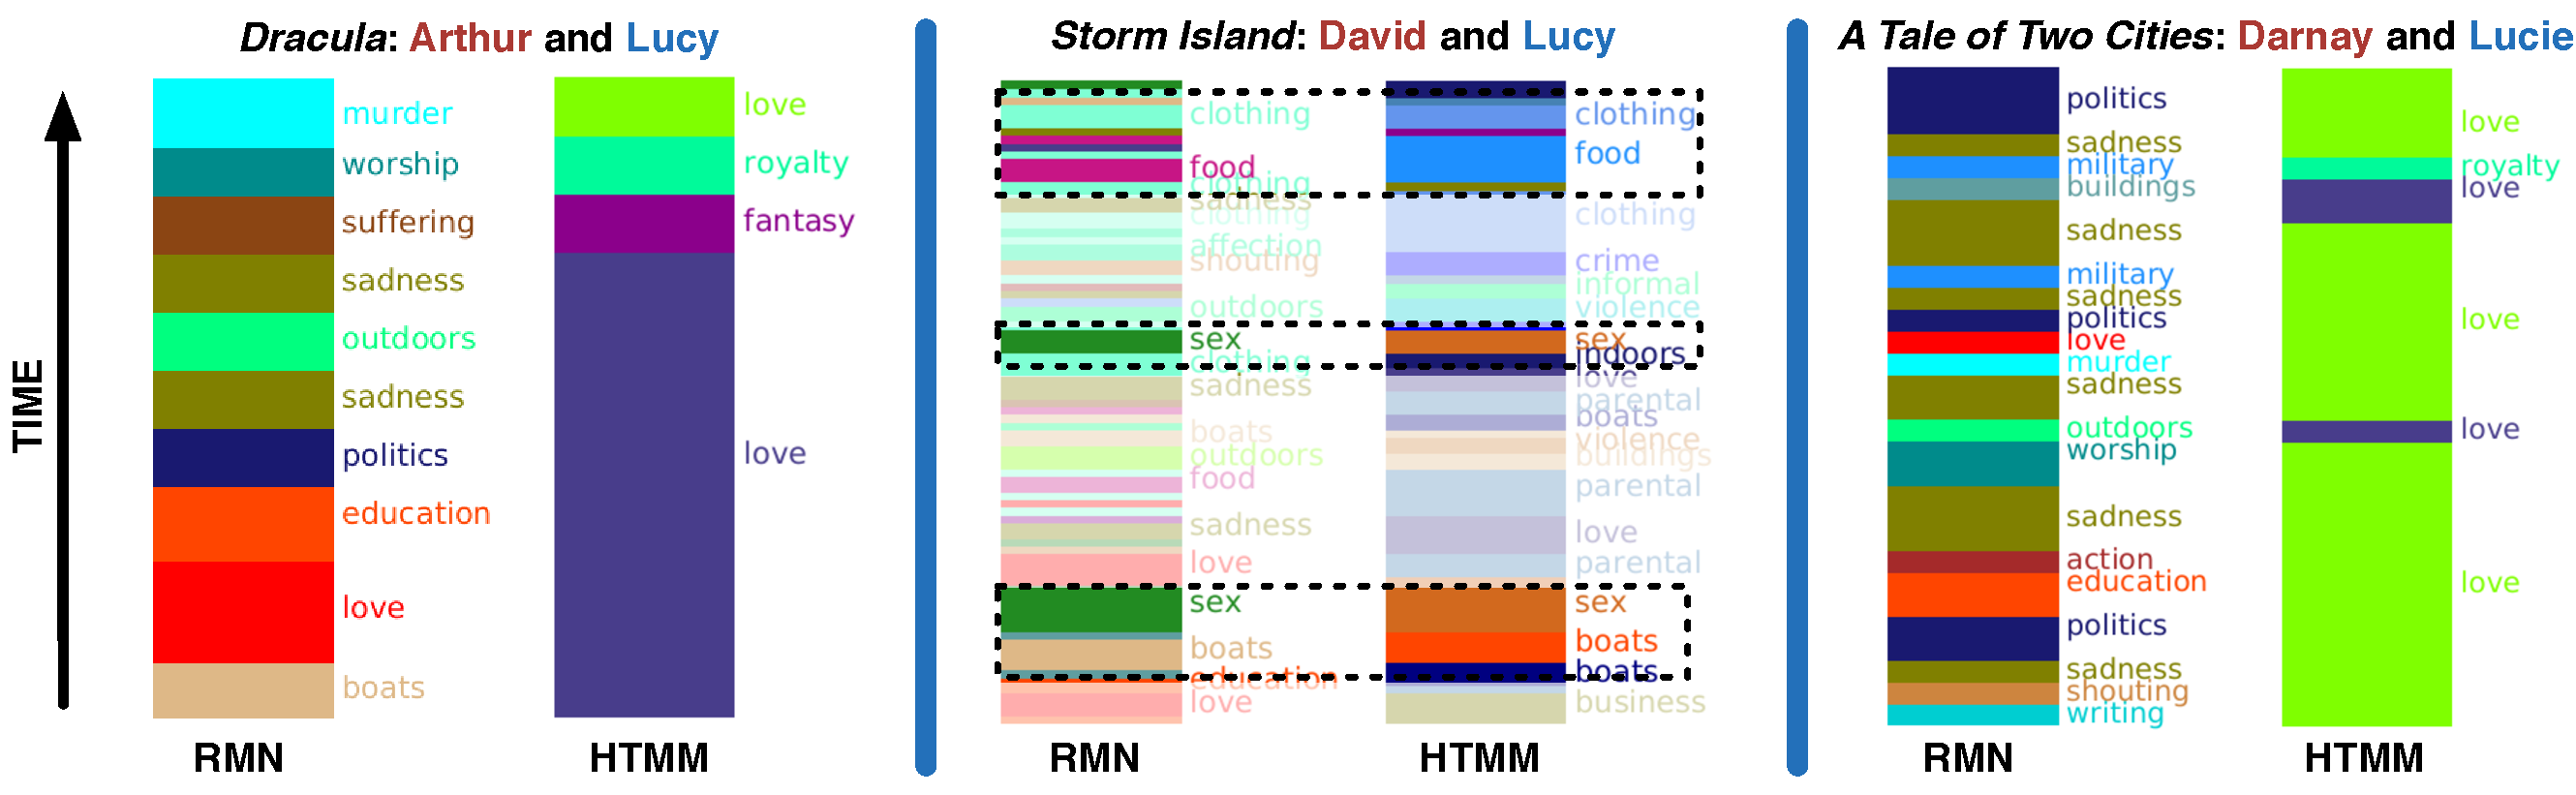
\includegraphics[width=1.0\linewidth]{2016_naacl_relationships/figures/good_bad_traj.pdf}
  \caption{\emph{Left}: the \rmn\ is able to model Arthur and Lucy's trajectory
    reasonably well compared to our manually-created version in
    Figure~\ref{fig:traj}. \emph{Middle}: both models agree on event-based
    descriptors such as \underline{food} and \underline{sex}. \emph{Right}: a
    failure case for the \rmn\ in which it is unable to learn that Lucie Manette
    and Charles Darnay are in love.}
\label{fig:goodbadtraj}
\end{figure*}

\begin{figure*}[ht]
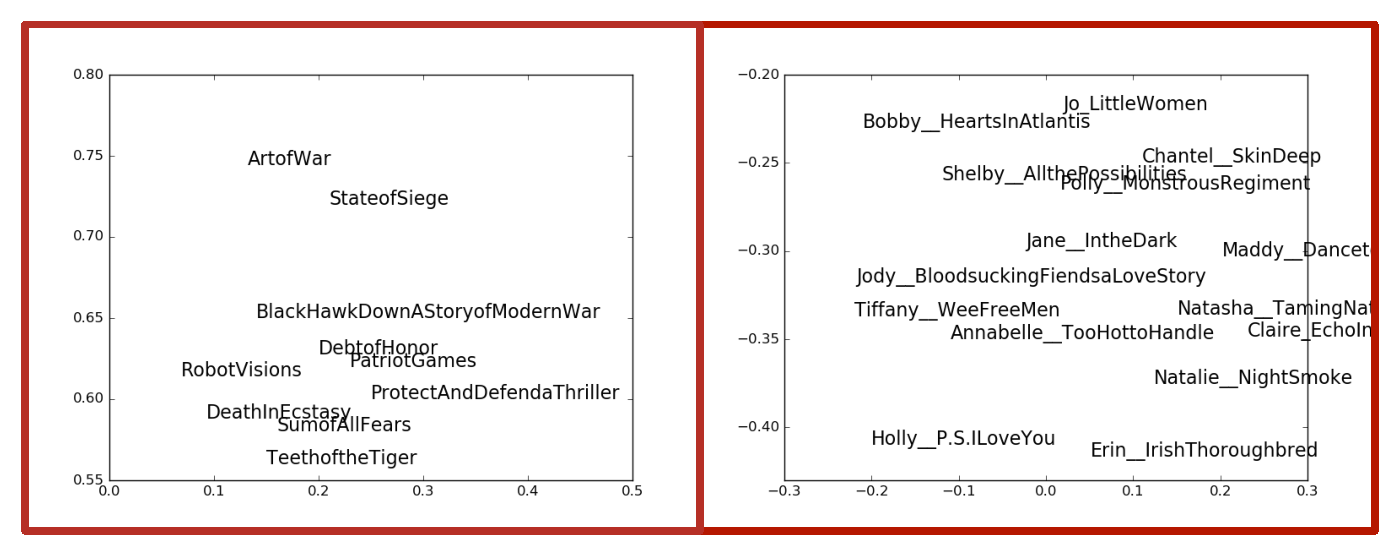
\includegraphics[width=1.0\linewidth]{2016_naacl_relationships/figures/charbookembeddings.pdf}
  \caption{Clusters from \abr{pca} visualizations of the \rmn's learned book (left) and character (right) embeddings. We see a cluster of books about war and violence (many of which are authored by Tom Clancy) as well as a cluster of lead female characters from primarily romance novels. These visualizations show that the \rmn\ can recover useful static representations of characters and books in addition to the dynamic relationship trajectories.}
\label{fig:bookpca}
\end{figure*}

Our experiments show the superiority of the \rmn\ over various topic model
baselines in both descriptor interpretability and trajectory accuracy, but what
causes the improved performance? In this section, we analyze similarities
between the \rmn\ and \htmm\ and look at qualitative examples where the
\rmn\ succeeds and fails. We also connect the findings of our affinity
experiment to existing literary scholarship.

Both models are equally proficient at learning and assigning event-based
descriptors (e.g., \underline{crime}, \underline{violence},
\underline{food}). More specifically, the \rmn\ and \htmm\ agree on
environmental descriptions (e.g., boats, outdoors) and graphic sexual scenes
(Figure~\ref{fig:goodbadtraj}, middle).

However, the \rmn\ is more sophisticated with interpersonal relationships. None
of the topic model baselines learns negative emotional descriptors such as
\underline{sadness} or \underline{suffering}, which explains the inaccurate
\htmm\ trajectory of Arthur and Lucy in the left-most panel of
Figure~\ref{fig:goodbadtraj}. All of the topic model baselines learn
duplicate topics; in Table~\ref{table:affinity}, one \underline{love} descriptor
is highly positive while a duplicate is strongly negative.\footnote{This
  ``duplicate love'' phenomenon persists even when we reduce the number of
  topics.} The \rmn\ circumvents this problem with its uniqueness penalty
(Equation~\ref{eq:unique}).

While the increased descriptor variety is a positive, sometimes it leads the
\rmn\ astray. The model largely ignores the love between Charles Darnay and
Lucie Manette in Dickens' \emph{A Tale of Two Cities} due to book's sad tone;
meanwhile, the \htmm's trajectory, while vastly simplified, does pick up on the
romance (Figure~\ref{fig:goodbadtraj}, right). While the \rmn's learnable book
and character embeddings should help, the signal in a span cannot lead to the
``proper'' descriptor.

Both the \rmn\ and \htmm\ learn that \underline{politics} is strongly negative
(Table~\ref{table:affinity}). Existing scholarship supports this finding:
Victorian-era authors, for example, are ``obsessed with \emph{otherness} \dots of
antiquated social and legal institutions, and of autocratic and/or dictatorial
abusive government''~\cite{zarifopol1995kill}, while in science fiction,
``dystopia—--precisely because it is so much more common (than utopia)—--bears
the aspect of lived experience''~\cite{gordin2010utopia}. Our affinity data
comes primarily from Victorian novels (e.g., by Dickens and George Eliot),
leading us to believe that that the models are behaving reasonably. Finally,
returning to the ``extra'' meaning of meals discussed in
Section~\ref{sec:introduction}, \underline{food} occurs
\emph{slightly} more frequently in positive relationships.
